\documentclass[10pt,a4paper]{report}
\usepackage[margin = 2.53cm]{geometry}
\usepackage[latin1]{inputenc}
\usepackage{amsmath}
\usepackage{wrapfig}
\usepackage{amsfonts}
\usepackage{graphicx}
\usepackage{amssymb}
\usepackage{rotating}
\usepackage{caption}
\usepackage{lscape}
\author{Daniel G. Holmes}

\begin{document}
\thispagestyle{empty}

\section*{Appendix A - UML Hierarchy Diagram}


\begin{figure}[h]
	\centering
		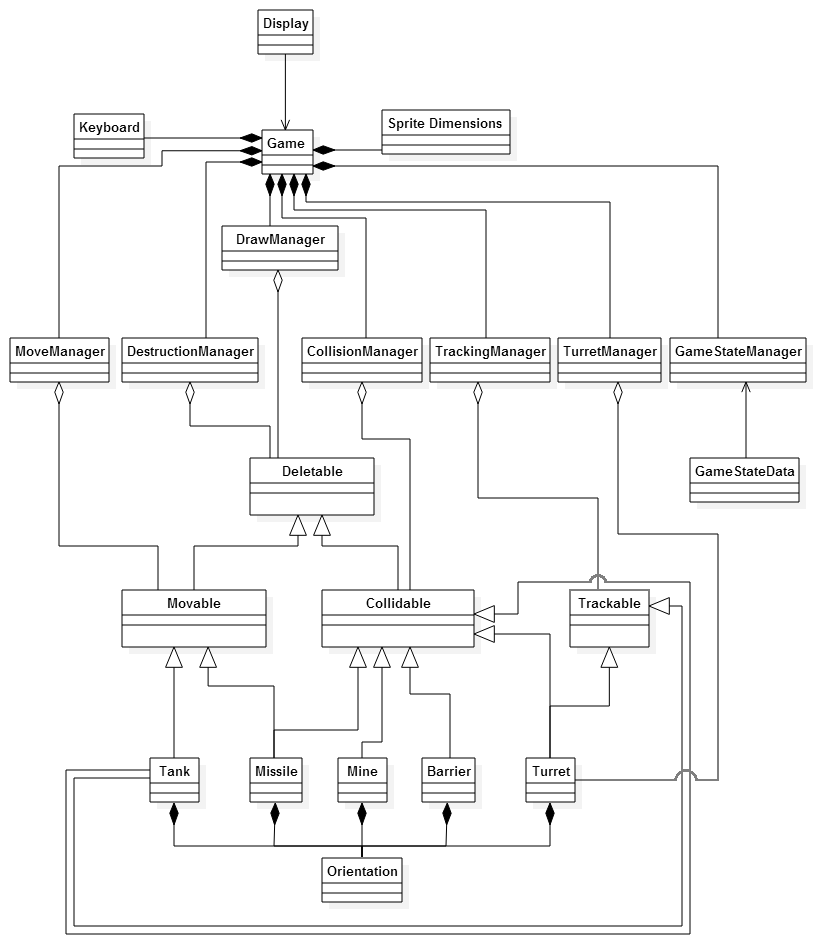
\includegraphics[keepaspectratio=true, scale=0.73]{uml-hierarchy}
	\label{top}
	\caption{UML Hierarchy of the game.}
	\setcounter{figure}{0}
\end{figure}

\newpage
\thispagestyle{empty}
\section*{Appendix B - Linking Program Layers}

\begin{figure}[h]
		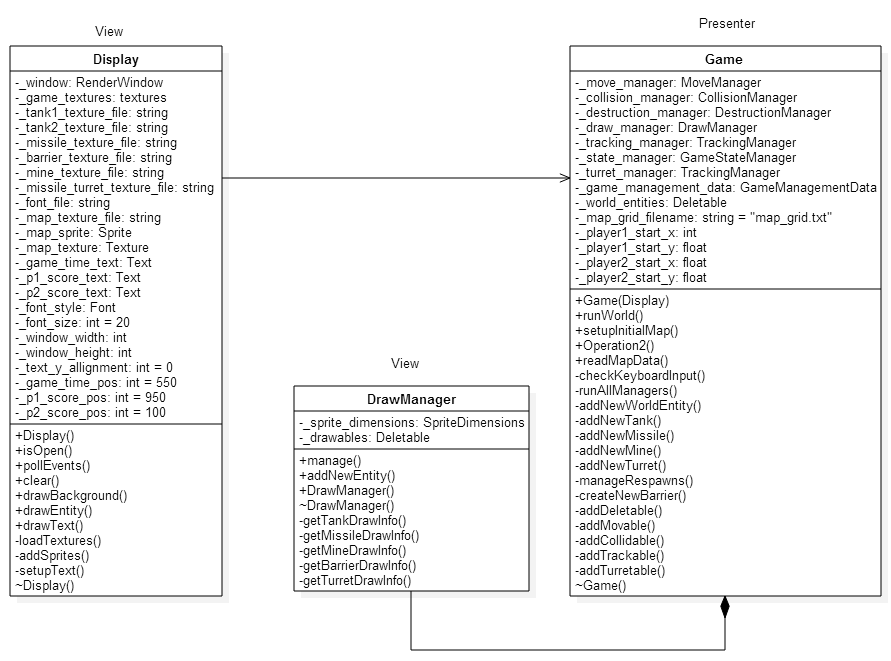
\includegraphics[keepaspectratio=true, scale=0.53]{uml-linking-layers}
	\label{top}
	\caption{UML diagram showing the linking of program layers.}
	\setcounter{figure}{0}
\end{figure}

\newpage
\thispagestyle{empty}
\begin{landscape}
\section*{Appendix C - Sequence Diagram}

\begin{figure}[h]
	\centering
		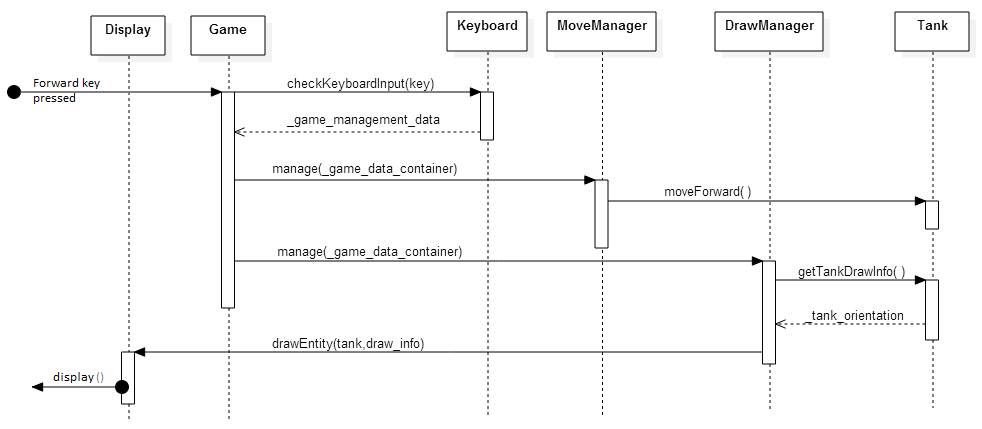
\includegraphics[keepaspectratio=true, scale=0.73]{sequence-diagram}
	\label{top}
	\caption{Example of the phases within a single program management cycle.}
	\setcounter{figure}{0}
\end{figure}


\newpage
\thispagestyle{empty}
\section*{Appendix D - Collision Detection Algorithm Performance}

\begin{figure}[h]
	\centering
		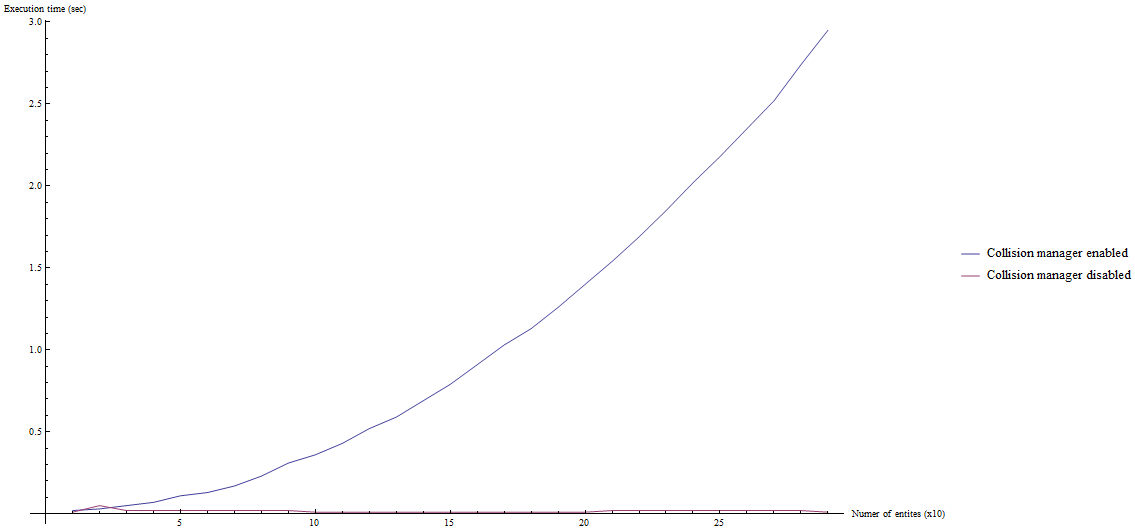
\includegraphics[keepaspectratio=true, scale=0.6]{timing-graphs}
	\label{top}
	\caption{Graph showing the performance of the collision detection algorithm.}
	\setcounter{figure}{0}
\end{figure}

\end{landscape}

\end{document}


